\documentclass[11pt,a4paper]{article}
\usepackage[margin=1in]{geometry}
\usepackage{amsmath,amssymb,amsthm}
\usepackage{xcolor}
\usepackage{booktabs}
\usepackage{longtable}
\usepackage{enumitem}
\IfFileExists{titlesec.sty}{%
  \usepackage{titlesec}%
  \titleformat{\section}{\large\bfseries\color{harborblue}}{\thesection}{0.7em}{}%
  \titleformat{\subsection}{\normalsize\bfseries}{\thesubsection}{0.6em}{}%
}{}
\usepackage[colorlinks=true,linkcolor=blue!45!black,urlcolor=blue!45!black]{hyperref}
\usepackage{tikz}
\IfFileExists{pgfplots.sty}{%
  \usepackage{pgfplots}%
  \pgfplotsset{compat=1.18}%
}{}
\usetikzlibrary{arrows.meta,positioning,fit,backgrounds,calc,shapes.geometric,shapes.symbols,decorations.pathmorphing,decorations.pathreplacing}
\definecolor{harborblue}{RGB}{30,70,110}
\definecolor{shipred}{RGB}{140,30,30}
\definecolor{seagreen}{RGB}{31,110,70}
\definecolor{slate}{RGB}{71,85,105}
\definecolor{slatedark}{RGB}{30,41,59}
\definecolor{amber}{RGB}{217,119,6}
\definecolor{emerald}{RGB}{16,185,129}
\newtheorem{theorem}{Theorem}
\newtheorem{claim}{Claim}
\theoremstyle{definition}
\newtheorem{change}{Change}
\newtheorem{move}{Move}
\theoremstyle{remark}
\newtheorem*{verdict}{Verdict}
\newtheorem*{adj}{Adjudication}
\setlist{itemsep=1pt,topsep=2pt}

% Shared native-figure styles for the harbor-research corpus (relation-maps,
% regime diagrams, and data plots). Vector TikZ/pgfplots only -- see
% docs/harbor-research/figures/CONVENTION.md for the house rule this follows.
\tikzset{
  relnode/.style={draw,rounded corners,thick,minimum width=2.6cm,minimum height=0.9cm,align=center,font=\small},
  relarrow/.style={-{Stealth[length=2.5mm]},thick},
  regimebox/.style={draw,thick,align=center,font=\small,inner sep=4pt},
}
\IfFileExists{pgfplots.sty}{%
\pgfplotsset{
  harbor curve/.style={
    width=0.46\textwidth,height=5.6cm,
    axis lines=left,
    label style={font=\scriptsize},
    tick label style={font=\scriptsize},
    title style={font=\small,align=center,yshift=2pt},
    legend style={font=\scriptsize,draw=black!25,fill=white,fill opacity=0.92,text opacity=1,rounded corners=1pt,inner sep=3pt},
    thick,
  },
  harbor bar/.style={
    width=0.46\textwidth,height=5.6cm,
    ybar,bar width=6pt,
    ymode=log,log origin=infty,
    axis lines=left,
    label style={font=\scriptsize},
    tick label style={font=\tiny},
    xticklabel style={rotate=40,anchor=east,font=\tiny,inner sep=1pt},
    title style={font=\small,align=center,yshift=2pt},
    legend style={font=\scriptsize,draw=black!25,fill=white,fill opacity=0.92,text opacity=1,rounded corners=1pt,inner sep=3pt},
  },
}
}{}

\usepackage{graphicx}
\graphicspath{{../figures/}}
\usepackage{mdframed}
\newmdenv[backgroundcolor=blue!4,linecolor=harborblue,linewidth=0.8pt,skipabove=6pt,skipbelow=6pt]{thebox}
\newmdenv[backgroundcolor=red!4,linecolor=shipred,linewidth=0.8pt,skipabove=6pt,skipbelow=6pt]{boundary}
\newcommand{\onebreath}[1]{\begin{center}\emph{#1}\end{center}}
\newcommand{\Ob}{\mathsf{O}}
\newcommand{\Fb}{\mathsf{F}}

\title{\textbf{What Needs an Authority}\\[4pt]
\large Mechanical Detection, Chartered Resolution, and the Exact Price of Sole Ownership\\[3pt]
\normalsize Paper 6 of the Harbor program: the coordination functions of a multi-agent harbor,\\
sorted into those an algorithm discharges and those a charter must pay for}
\author{Prepared for Erich Owens}
\date{August 2026}
\begin{document}
\maketitle

\begin{abstract}
\noindent Multi-agent governance documents hand out authorities freely: a \emph{lookout} that scans incoming commitments for
conflicts, a \emph{sole owner} for the roadmap, the test suite, the release tag. This paper asks which of those coordination
functions genuinely require a designated authority, and prices the ones that do. Two results. First, conflict \emph{detection} needs
no authority at all --- inside a designed commitment fragment $\mathcal{L}_c$ (definite Horn rules with $\bot$ heads, ground deontic
obligation/prohibition rules over scopes and intervals, exclusive interval claims, difference constraints), detection is a
polynomial, witness-producing algorithm, $O(H + T\log T + C\log C + V\!\cdot\!E)$, validated against a brute-force oracle on 3000
random policy sets with zero disagreements; and composed with the supervisory-control theorem of Paper 2 it is not even a role, but
a guard: acceptance is a mediated write, so in-fragment conflict-freedom is \emph{regimentable} --- the runtime refuses the commit.
One expressive step outside the fragment (disjunctive obligations under discharge choice), conflict-freedom is NP-complete, and
\emph{there} an authority becomes necessary: not to notice the conflict but to choose the discharge. Second, sole \emph{ownership}
of a role is not a principle but an inequality: a sole specialist beats a pooled swarm exactly when the skill premium clears the
Erlang-C boundary $g_A(\rho,c)$ --- the whitepaper's proposed threshold is falsified in both directions, with the two thresholds
crossing at $\rho=(3-\sqrt5)/2$ --- and a sole owner who can die and be succeeded is viable at \emph{any} skill premium only while
the death-rate--times--succession-time product stays below $D^\star=\eta K/(1-\eta K)$: past that line, pooling wins even against an
infinitely skilled specialist. The slogan the two theorems earn: an authority is needed exactly where the algorithm ends, and where
it is needed, its price is a computable number, not a vibe.
\end{abstract}

\vspace{0.5em} \noindent\textbf{Express lane.} \emph{Conflict detection inside the designed commitment fragment is polynomial and
witness-producing (no judge consumed, and via Paper 2 the check is enforceable pre-commit by the runtime); one disjunctive
obligation outside the fragment makes conflict-freedom NP-complete, which is where a chartered resolver must choose; and sole
ownership of a role pays iff $\mu_s/\mu_g \ge g_A(\rho,c)$ --- exact Erlang-C form in the box of \S\ref{sec:thm-boundary} --- with
sole-owner viability capped at $\xi/\eta \le D^\star$ absent skill limits.} Experts: read the two boxes
(\S\ref{sec:thm-detect}, \S\ref{sec:thm-boundary}), the succession box (\S\ref{sec:succession}), and the inventory table
(\S\ref{sec:inventory}); the rest is scaffolding.

\section{The scene: the harbor's authority inventory}\label{sec:scene}
A harbor of coding agents runs on commitments: standing prohibitions (\emph{never write to prod}), conditional obligations
(\emph{if you deploy, you must update the runbook within the window}), exclusive claims (\emph{this file is mine from tick 5 to
tick 20}), deadlines chained to deadlines. The governance document responds with authorities. A \emph{lookout} is chartered to
scan every proposed commitment against the accepted set and reject contradictions. \emph{Sole-responsibility roles} --- a roadmap
owner, a test-suite curator, a release avatar --- each hold exclusive write capability over one invariant, on the theory that a
single deeply-skilled owner beats a committee.

Both assignments feel natural, and both smuggle in an unexamined premise: that the function \emph{requires a designated authority}
--- a mind with standing, judgment, and a name --- rather than a subroutine and a price. The operations lead's two questions are
therefore exact. \emph{Does the lookout need judgment, or is contradiction-scanning mechanical?} And \emph{when does the sole
owner actually beat the pool --- and what happens when the owner dies mid-quarter?} This paper answers both with theorems that were
run before they were believed: the first by a 3000-instance oracle sweep with zero disagreements [internal,
\texttt{b4\_deontic\_fragment.py}], the second by a sweep that \emph{falsified the whitepaper's own proposed threshold in both
directions} before replacing it [internal, \texttt{b8\_specialization.py}].

\paragraph{The idea in one breath.}
\onebreath{An authority is needed exactly where the algorithm ends: inside a designed commitment fragment, conflict detection is a
polynomial witness-producing decision the runtime can enforce pre-commit --- no judge; one expressive step outside, conflict-freedom
is NP-complete and a chartered resolver must choose; and sole ownership of a role is justified not by principle but by an exact
Erlang-C threshold on skill, payable only while the owner's death-rate--times--succession-time stays below $D^\star$.}

\paragraph{Intuition: the working port.} Watch a real port for a day (Figure~\ref{fig:relation}). Whether two vessels are on a
collision course is \emph{geometry} --- constant bearing, decreasing range --- computed identically by every watch officer;
nobody's authority is consulted. Who gives way is next decided by a \emph{rulebook} (the collision regulations) --- still
mechanical, still nobody's judgment. Only where the rulebook ends --- a three-vessel crossing the rules never anticipated --- does
harbor traffic control exercise chartered discretion. And the port's one genuinely personal authority, the licensed pilot with
twenty years on these shoals, is hired against a pool of tug crews only when the water is hard enough to pay the premium ---
and the port licenses a second pilot, because a port whose only pilot can fall ill has priced its channel's availability at one
human body. The structural mapping: collision geometry $\to$ in-fragment conflict detection (mechanical, witness-producing);
the rulebook's edge $\to$ the fragment's NP-complete frontier (where chartered resolution begins); the pilot's premium and the
second license $\to$ the $g_A(\rho,c)$ boundary and the succession price $D^\star$. The analogy maps relations, so it earns a
prediction: making the rulebook \emph{richer} should eventually make rule-following itself intractable and reintroduce discretion
--- and that is exactly what the NP-completeness theorem says happens one disjunction past the fragment.

The predictable misread, preempted: \emph{mechanical detection does not mean mechanical governance}. The checker certifies the
norm \emph{system}, never the norms --- a bad policy consistently held is consistent --- and detection without a resolution charter
just produces alarms. The theorems do not abolish authority; they \emph{relocate} it, from noticing to choosing, and then hand the
remaining authority its bill.

\begin{figure}[t]\centering 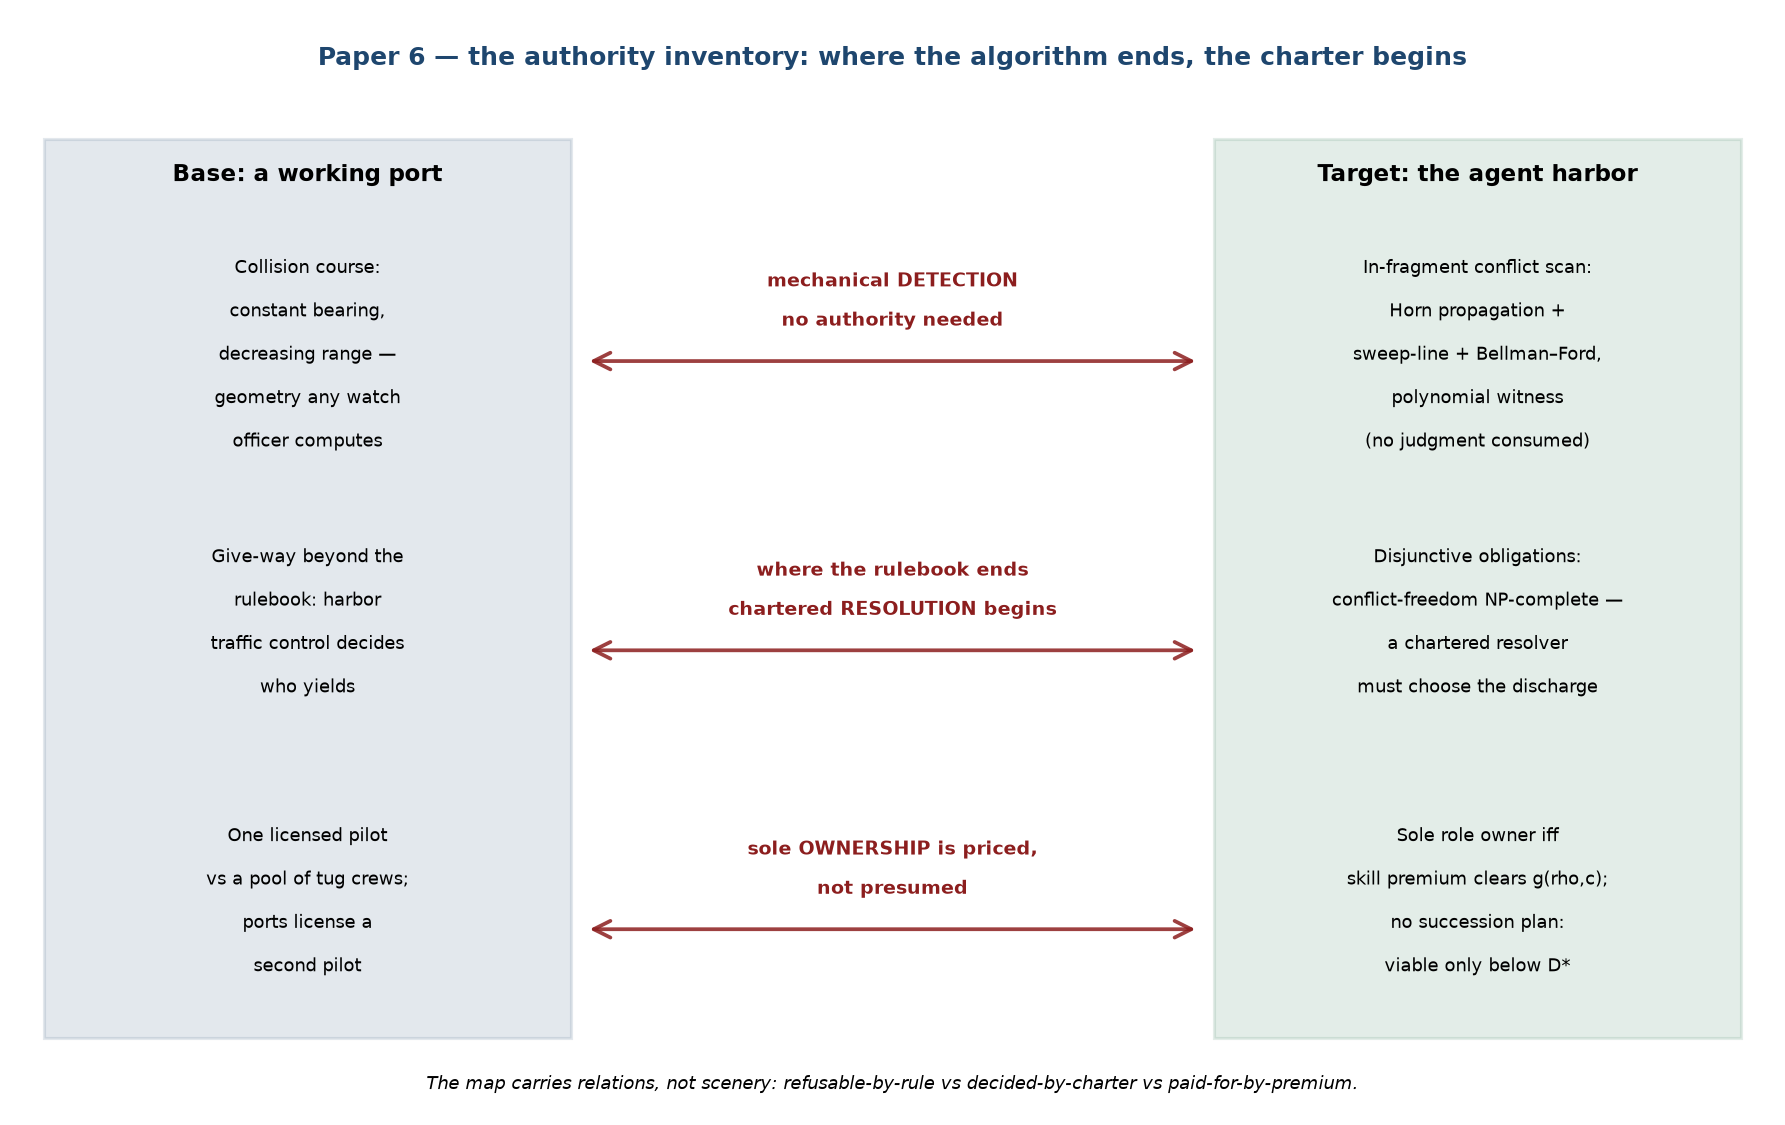
\includegraphics[width=0.96\textwidth]{paper6_relation.png}
\caption{The relation map. Base domain: a working port --- collision-course detection is geometry, give-way beyond the rulebook is
harbor traffic control's chartered call, and the sole licensed pilot is paid a premium against a pool of tug crews, with a second
license mandated. Target domain: the agent harbor --- in-fragment conflict scanning is Horn propagation + sweep-line +
Bellman--Ford with a polynomial witness; disjunctive obligations make conflict-freedom NP-complete, so a chartered resolver
chooses the discharge; and a sole role owner is justified iff the skill premium clears $g_A(\rho,c)$, with no-succession viability
capped at $D^\star$. The correspondence arrows carry the theorem content: refusable-by-rule vs decided-by-charter vs
paid-for-by-premium.}
\label{fig:relation}\end{figure}

\section{Part I. The lookout is a subroutine: the fragment $\mathcal{L}_c$}\label{sec:lang}
Cheap detection is a \emph{language-design} choice, not a discovery about deontic logic in general. The commitment language
$\mathcal{L}_c$ buys it by construction. A policy set in $\mathcal{L}_c$ contains: \begin{itemize}
\item \textbf{facts} (ground atoms) and \textbf{definite Horn rules} $a_1\wedge\dots\wedge a_k \to b$, where the head $b$ may be
the contradiction symbol $\bot$;
\item \textbf{deontic rules} $\mathrm{body} \to \mathsf{M}(\mathrm{act}, s, [t_1,t_2])$ with $\mathsf{M}\in\{\Ob,\Fb\}$: when the
(Horn) body holds, action $\mathrm{act}$ is obliged or forbidden on scope atoms $s$ over the ground time interval $[t_1,t_2]$;
\item \textbf{exclusive interval claims} (\emph{resource $x$ is exclusively mine on $[t_1,t_2]$});
\item \textbf{difference constraints} $x_j - x_i \le c$ over deadline variables.
\end{itemize}
A \emph{conflict} is any of four things: derivable $\bot$; a fired $\Ob$/$\Fb$ pair on the same action with overlapping
scope-and-interval; two exclusive claims overlapping on the same resource; or a negative cycle in the difference-constraint graph
(an unsatisfiable deadline system). This is deliberately a \emph{ground} fragment --- no nesting of deontic operators, no
negation-as-failure, monotone bodies only --- and \S\ref{sec:related} says explicitly which classical deontic puzzles are thereby
left outside the door.

\section{The detection theorem and its frontier}\label{sec:thm-detect}
\begin{thebox}
\textbf{Theorem 1a (membership: detection is polynomial and witness-producing).} For a policy set in $\mathcal{L}_c$ with Horn
program size $H$, $T$ fired deontic tokens, $C$ exclusive claims, and difference-constraint graph $(V,E)$, conflict detection is
decidable in $O(H + T\log T + C\log C + V\!\cdot\!E)$, with a polynomial witness per conflict: Dowling--Gallier unit propagation
computes the least Horn model in $O(H)$ --- which by monotonicity equals the intersection of all models, i.e.\ exactly the
statuses forced in \emph{every} world [verified framework, Dowling--Gallier 1984]; a keyed sweep-line over interval endpoints
finds every $\Ob$/$\Fb$ clash and claim overlap in $O(T\log T + C\log C)$; Bellman--Ford returns a negative cycle iff the deadline
system is infeasible, in $O(V\!\cdot\!E)$. The witnesses are, respectively: a derivation chain, the two fired rules with their
overlap interval, the two claims, and the negative cycle.

\textbf{Theorem 1b (frontier: one step outside is NP-complete).} Extend $\mathcal{L}_c$ with disjunctive obligations
$\Ob(l_1\vee\dots\vee l_k)$ under discharge-choice semantics (the agent picks which disjunct to discharge). Conflict-freedom of a
policy set becomes NP-complete: membership by the selection certificate; hardness from 3-SAT --- each variable $x$ becomes a pair
of deontic rules $\mathrm{sel}_x^{+} \to \Ob(\mathrm{assert}_x)$ and $\mathrm{sel}_x^{-} \to \Fb(\mathrm{assert}_x)$ on
\emph{identical} scope and interval, each clause becomes a disjunctive obligation over its selector literals, and a conflict-free
discharge selection exists iff the formula is satisfiable [verified: reduction restated here in full; checked both directions on
16/16 instances, internal, \texttt{b4\_deontic\_fragment.py}].
\end{thebox}

\paragraph{Verification.} 3000 random in-fragment policy sets against a brute-force oracle (all $2^5$ Horn models intersected;
pairwise overlap checks; exhaustive integer search over the complete potential box $[-\Sigma|c|,0]^V$ for the difference system):
885 conflicts found --- 121 derivable $\bot$, 195 $\Ob$/$\Fb$ clashes, 484 claim overlaps, 213 negative temporal cycles --- of
which 149 are reachable \emph{only} through Horn propagation; \textbf{0 disagreements} with the oracle, and least model $=$
intersection-of-all-models on all 3000 [internal, \texttt{b4\_deontic\_fragment.py}, seed 20260816]. The 3-SAT reduction was
verified in both directions on 8 satisfiable and 8 unsatisfiable random instances ($n{=}4$, $m{=}7$--$28$), 16/16, with the
satisfying assignment extracted from each conflict-free selection. Mutation: deleting Horn propagation (checking only directly
stated statuses) misses 100 of the 885 sweep conflicts --- propagation is load-bearing at scale, not a formality [internal].

\paragraph{Numbers by hand.} The mutant's canonical miss is a four-line policy a reviewer can check aloud: fact
\texttt{deploy}; Horn rule $\texttt{deploy} \to \texttt{prod\_access}$; deontic rule $\texttt{prod\_access} \to
\Ob(\texttt{write\_prod}, s, [5,10])$; standing $\Fb(\texttt{write\_prod}, s, [0,20])$. Propagation forces
\texttt{prod\_access}, the obligation fires, and the sweep-line reports the $\Ob$/$\Fb$ overlap on $[5,10]\cap[0,20]=[5,10]$ ---
while a pairwise scanner that never propagates sees no directly stated clash and stays silent [internal, the printed witness].
For the frontier, run the reduction on the smallest unsatisfiable formula $(x)\wedge(\neg x)$: two disjunctive obligations force
both $\mathrm{sel}_x^{+}$ and $\mathrm{sel}_x^{-}$, firing $\Ob(\mathrm{assert}_x)$ and $\Fb(\mathrm{assert}_x)$ on identical
scope and interval --- every selection conflicts, matching unsatisfiability [verified: two lines]. \emph{Now you try:} facts
$\{\texttt{audit\_open}\}$; rules $\texttt{audit\_open} \to \texttt{vault\_access}$ and $\texttt{vault\_access} \to
\Ob(\texttt{read\_ledger}, s, [2,6])$; standing $\Fb(\texttt{read\_ledger}, s, [4,9])$. Conflict? (Yes: propagation forces
\texttt{vault\_access}, the obligation fires, and the overlap is $[4,6]$ --- a two-hop indirect conflict, exactly the species the
mutant misses.)

\section{Composition with Paper 2: the lookout is not even a role}\label{sec:regiment}
Paper 2 proved that a safety policy over an agent's event alphabet is enforceable-by-prevention (\emph{regimentable}) iff it is
Ramadge--Wonham controllable --- no uncontrollable event carries a legal history out of the policy --- and its design rule was:
uncontrollable events in a policy's \emph{condition} are free; only uncontrollable events in its \emph{prohibition} are fatal.
Now compose. In the harbor, \emph{acceptance of a commitment is a mediated write}: the accepted set lives in the single-writer
store, and the acceptance event is a member of $\Sigma_c$, the controllable alphabet. The policy \emph{``never accept a proposal
whose union with the accepted set conflicts in-fragment''} therefore gates a controllable event on a condition that Theorem~1a
makes a total, polynomial-time-computable predicate of committed state. The policy is controllable, hence regimentable: the
conflict never enters the accepted set, because the daemon refuses the write, with the theorem's witness attached to the refusal
[verified: composition of Theorem 1a with Paper 2's boxed theorem; both components machine-checked separately, internal,
\texttt{b4\_deontic\_fragment.py} $+$ \texttt{b3\_controllability.py}].

This is the paper's first answer, and it is sharper than ``the lookout doesn't need judgment.'' Inside the fragment the lookout is
not an authority at all --- it is a \emph{guard clause} at the mediation boundary, as impersonal as a type check, producing a
four-line witness instead of a verdict. What the charter must still supply is everything the guard cannot: \emph{which} of two
conflicting proposals yields (priority, negotiation, waiver), \emph{whether} a standing norm should be amended, and --- the moment
anyone wants disjunctive obligations --- \emph{which discharge to choose}, because Theorem~1b says no proposal-time check scales
there unless P$=$NP. The frontier is thus the exact line where authority re-enters: the schema designer reads Theorem~1 as a price
list --- keep the language in $\mathcal{L}_c$ and detection is a regimentable subroutine; buy the expressive convenience of
disjunction and you have hired a judge, with a queue.

\section{Part II. The sole owner: an inequality, not a principle}\label{sec:queue}
The whitepaper's sole-responsibility roles (roadmap owner, test-suite curator, release avatar) trade pooled capacity for
accountability and skill. Model the trade honestly. Requests for the invariant-critical function arrive Poisson at rate
$\lambda$; a sole specialist serves them as an $M/M/1$ queue at rate $\mu_s$; the pooled alternative is an $M/M/c$ queue of
generalists at rate $\mu_g$ each, utilization $\rho=\lambda/(c\mu_g)$; the skill premium is $r=\mu_s/\mu_g$. Sole ownership also
carries an \emph{accountability value} $A$ (the worth of single-writer attribution per unit time of demand) against a waiting
cost $w$ per request-hour. The whitepaper proposed the threshold $\tilde g = 1+(c-1)\rho/(1-\rho)$ and marked it \emph{status:
proposed}. The sweep ran before the belief formed --- and falsified $\tilde g$ in both directions.

\section{The specialization boundary}\label{sec:thm-boundary}
\begin{thebox}
\textbf{Theorem 2 (queueing specialization boundary).} With $C(c,\rho)$ the Erlang-C delay probability, sole ownership weakly
dominates the pool in net cost iff the skill premium clears
\[ \frac{\mu_s}{\mu_g} \;\ge\; g_A(\rho,c) \;=\; c\rho \;+\;
\frac{1}{\,1 + \dfrac{C(c,\rho)}{c(1-\rho)} + \dfrac{A\mu_g}{w\lambda}\,}, \]
reducing at $A=0$ to $g(\rho,c) = c\rho + \dfrac{c(1-\rho)}{c(1-\rho)+C(c,\rho)}$, with $g(\rho,1)=1$ (a specialist against one
generalist needs no premium), $g\to c$ as $\rho\to 1$ (the boundary \emph{saturates} at the capacity ratio, never diverges), and
the closed form $g(\rho,2)=1+2\rho-\rho^2$ [verified: derivation below]. The proposed threshold
$\tilde g = 1+(c-1)\rho/(1-\rho)$ is \textbf{falsified in both directions}: at $c{=}2,\rho{=}0.1,r{=}1.15$ it certifies a
specialist who loses ($W_{\mathrm{solo}}=1.0526 > W_{\mathrm{pool}}=1.0101$; simulation $z=-15.7$), at
$c{=}2,\rho{=}0.5,r{=}1.9$ it rejects a specialist who wins ($1.111 < 1.333$; $z=+32$); the two thresholds cross at
$\rho=(3-\sqrt5)/2\approx0.382$, and where $g$ saturates $\tilde g$ diverges ($\rho{=}0.9, c{=}8$: $g=7.73$ vs $\tilde g=64$)
[internal, \texttt{b8\_specialization.py}, seed 20260816].
\end{thebox}

\paragraph{Numbers by hand.} The theorem is two lines of algebra on textbook formulas, which is the right way to first believe
it. Sole ownership pays iff $w\lambda(W_{\mathrm{solo}}-W_{\mathrm{pool}}) \le A$, i.e.\ $1/(\mu_s-\lambda) \le W_{\mathrm{pool}}
+ A/(w\lambda)$; invert and divide by $\mu_g$, using $\lambda/\mu_g = c\rho$ and $\mu_g W_{\mathrm{pool}} = 1 +
C(c,\rho)/(c(1-\rho))$, and $g_A$ falls out [verified]. For $c=2$ the Erlang-C value is $C(2,\rho)=2\rho^2/(1+\rho)$, so
$c(1-\rho)/(c(1-\rho)+C) = (1-\rho^2)/((1-\rho^2)+\rho^2) = 1-\rho^2$ and $g(\rho,2) = 2\rho + 1 - \rho^2$ [verified: three
lines]. Now check the falsification instances by hand at $\mu_g=1$. At $\rho=0.1$: $g=1+0.2-0.01=1.19$ while
$\tilde g=1+0.1/0.9=1.111$, so $r=1.15$ sits between them --- the whitepaper certifies, the truth rejects; indeed
$W_{\mathrm{solo}}=1/(1.15-0.2)=1.0526$ against $W_{\mathrm{pool}}=1+0.0182/1.8=1.0101$ [verified]. At $\rho=0.5$:
$g=1.75$, $\tilde g=2$, and $r=1.9$ again sits between --- rejected by the whitepaper, but
$W_{\mathrm{solo}}=1/0.9=1.111 < W_{\mathrm{pool}}=4/3$ [verified]. Setting $1+2\rho-\rho^2 = 1+\rho/(1-\rho)$ gives
$\rho^2-3\rho+1=0$: the thresholds cross at $\rho=(3-\sqrt5)/2$, which is why the falsification runs in \emph{both} directions
--- Figure~\ref{fig:regime}, Panel A, shades the two error lenses [verified]. \emph{Now you try:} at $c{=}2$, $\rho{=}0.3$, does $r=1.5$ justify a sole owner? ($g(0.3,2)=1+0.6-0.09=1.51$ --- no,
by a hair; $\tilde g=1.43$ would have said yes. The flattering threshold flatters exactly below the crossing.)

The cross-validation stack behind the closed forms: Erlang-C means against discrete-event simulation, $|z|\le1.8$ across the
grid; the 60-instance random sweep over $(\lambda,\mu_s,\mu_g,c,A,w,\xi,\eta)$ gave 55 decisive instances and \textbf{0} sign
violations of the boundary [internal, \texttt{b8\_specialization.py}].

\begin{figure}[t]\centering 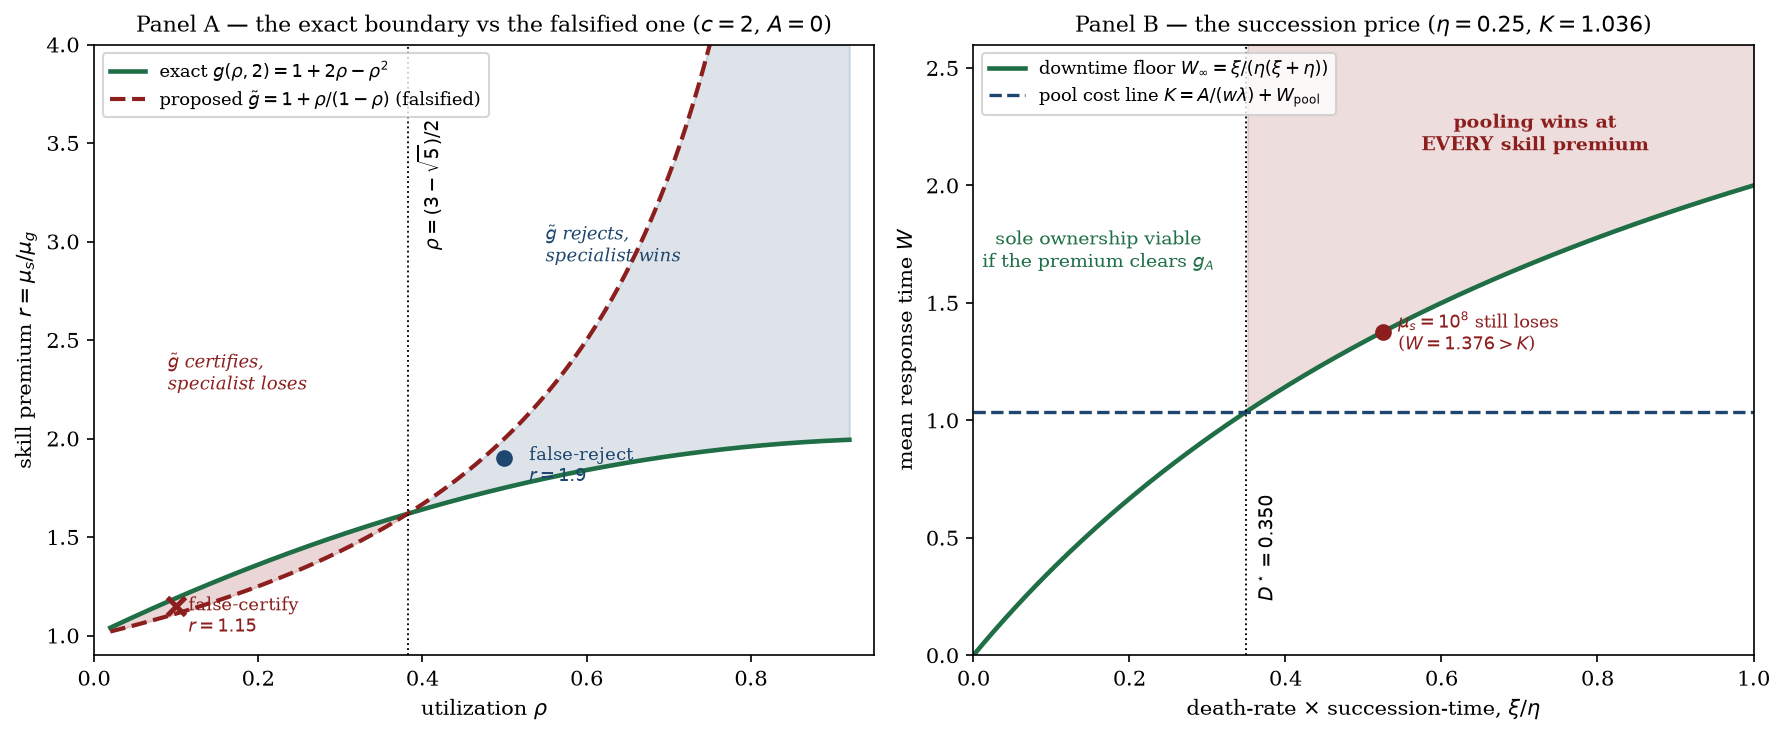
\includegraphics[width=0.98\textwidth]{paper6_regime.png}
\caption{The regime diagram. Panel A: the exact boundary $g(\rho,2)=1+2\rho-\rho^2$ (solid) against the falsified proposal
$\tilde g$ (dashed); the shaded lenses are the two error regimes --- false-certify below the crossing at $\rho=(3-\sqrt5)/2$,
false-reject above it --- with the two refuting instances marked ($r{=}1.15$ at $\rho{=}0.1$; $r{=}1.9$ at $\rho{=}0.5$). Panel B:
the succession price at the reference instance ($\eta{=}0.25$, $K{=}1.036$): the downtime floor $W_\infty=\xi/(\eta(\xi+\eta))$
crosses the pool cost line at $D^\star=0.350$; to its right pooling wins at every skill premium --- the marked point is a
$\mu_s=10^8$ specialist still losing at $\xi/\eta=1.5D^\star$ ($W=1.376>K$). Both panels regenerate from
\texttt{b8\_specialization.py} [internal, seed 20260816].}
\label{fig:regime}\end{figure}

\section{The succession price: what one mortal body costs}\label{sec:succession}
The boundary above assumes the specialist never disappears. Sole owners disappear: sessions die, containers are reaped,
providers churn. Model the corner honestly: the specialist \emph{dies} at rate $\xi$ and is \emph{succeeded} after an
$\mathrm{Exp}(\eta)$ spin-up (context transfer, warm-up, credential rebinding), work resuming where it stopped, requests
queueing throughout --- an $M/M/1$ queue with breakdowns in the Mitrany--Avi-Itzhak lineage.

\begin{thebox}
\textbf{Theorem 3 (price of the succession rule).} With effective rate $\mu_{\mathrm{eff}}=\mu_s\eta/(\xi+\eta)$, the sole
owner's mean response time is exactly
\[ W_{\mathrm{bd}} \;=\; \frac{1+\mu_s\xi/(\xi+\eta)^2}{\mu_{\mathrm{eff}}-\lambda}
\;=\; \frac{1}{\mu_{\mathrm{eff}}-\lambda} \;+\; \frac{\mu_{\mathrm{eff}}}{\mu_{\mathrm{eff}}-\lambda}\,W_\infty,
\qquad W_\infty=\frac{\xi}{\eta(\xi+\eta)}, \]
decreasing in $\mu_s$ with infimum $W_\infty$: \emph{no amount of skill buys back residual downtime}. Consequently, with
$K = A/(w\lambda) + W_{\mathrm{pool}}$ the pool's cost line, pooling dominates at \emph{every} skill premium iff
\[ \frac{\xi}{\eta} \;>\; D^\star \;=\; \frac{\eta K}{1-\eta K}, \]
and $D^\star$ is the price of the succession rule: a sole role without a succession plan (small $\eta$) is viable only while its
death-rate--times--succession-time product stays below $D^\star$ [verified: $W_\infty(\xi^\star)=K$ at
$\xi^\star=D^\star\eta$ is one line of algebra; closed form checked against matrix-geometric solution to $2\times10^{-13}$,
truncated CTMC to $10^{-14}$, Gillespie simulation $|z|\le0.8$, internal, \texttt{b8\_specialization.py}].
\end{thebox}

\paragraph{Numbers by hand.} Reference instance: $\lambda{=}1$, $c{=}4$, $\mu_g{=}1.2$ (so $\rho=0.208$), $A{=}0.2$, $w{=}1$,
$\eta{=}0.25$. Erlang-C gives $C(4,0.208)=0.0110$, so $W_{\mathrm{pool}}=1/1.2+0.0110/(4\cdot1.2\cdot0.792)=0.8362$ and
$K=0.2+0.8362=1.0362$ [verified: four-function-calculator arithmetic on the boxed formulas]; then $\eta K = 0.2591$ and
$D^\star = 0.2591/0.7409 = 0.350$ [verified]. Just past the line, at $\xi/\eta = 1.5\,D^\star$, an absurdly skilled specialist
($\mu_s=10^8$) still loses: $W=1.376 > K=1.036$ --- the floor $W_\infty$, not the skill, is binding [internal]. The identity in
the box also explains the program's recorded wrong turn: the naive decomposition $W_{\mathrm{bd}} =
1/(\mu_{\mathrm{eff}}-\lambda) + W_\infty$ is refuted (it predicts $4.17$ where the truth is $8.17$ at the canary instance
$\mu_s{=}5$, $\xi{=}0.5$), because downtime also \emph{builds queue}: the residual is amplified by
$\mu_{\mathrm{eff}}/(\mu_{\mathrm{eff}}-\lambda) = 2.5$ there, and $1.5 + 2.5\times2.667 = 8.17$ checks by hand [verified
arithmetic; refutation internal]. Panel B of Figure~\ref{fig:regime} draws exactly this geometry: the floor $W_\infty$ crossing
the pool cost line at $D^\star$. \emph{Now you try:} at the reference instance, is a sole owner with a same-day succession plan
($\eta=2$; $K$ is unchanged at $1.0362$, so $\eta K = 2.07 > 1$) ever capped? (No: $\eta K \ge 1$ makes $D^\star=\infty$ --- a
fast enough succession plan removes the viability ceiling entirely, leaving only the Theorem-2 premium test. That is what a
succession plan \emph{buys}.)

The implementation hazard is also priced. A cost model that forgets breakdowns entirely (plain $M/M/1$) is caught by the
high-$\xi$ canary: at $\xi/\eta=2 \gg D^\star$, the mutant says SPECIALIST while simulation says the pool wins decisively
($\Delta C = -7.06 \pm 0.16$); at low $\xi$ the mutant is indistinguishable --- so the canary, not routine testing, is what makes
the omission visible [internal, \texttt{b8\_specialization.py}].

The predictable misread, preempted: $D^\star$ does not say specialists are bad, and Theorem 2 does not say pooling is the
default truth. Together they say sole ownership is a \emph{purchase}: below the boundary the premium does not cover the
congestion cost and the honest ledger entry is ``we pay latency $w\lambda(W_{\mathrm{solo}}-W_{\mathrm{pool}})-A$ per unit time
for accountability''; above $D^\star$ the purchase is unavailable at any price until the succession plan (larger $\eta$) is
bought first. Every quantity in both tests --- $\lambda$, $\mu_s$, $\mu_g$, $\xi$, $\eta$ --- is daemon-metered, so the harbor
can re-grade its roles from telemetry rather than from taste.

\section{The authority inventory, priced}\label{sec:inventory}
The two parts assemble into the answer to the title question:

\begin{center}\begin{tabular}{@{}p{0.36\textwidth}p{0.2\textwidth}p{0.36\textwidth}@{}}
\toprule
Coordination function & Authority needed? & What it costs \\
\midrule
In-fragment conflict detection & none (algorithm) & $O(H+T\log T+C\log C+V\!\cdot\!E)$ per batch, witness included \\
In-fragment conflict enforcement & none (runtime guard) & mediated acceptance write; regimentable via Paper 2 \\
Conflict-freedom with disjunctive obligations & chartered resolver & NP-complete check, or a judge who chooses the discharge \\
Priority, waiver, norm amendment & chartered, irreducibly & outside every checker; the charter's residual job \\
Sole ownership of a role & conditional & justified iff $r \ge g_A(\rho,c)$; otherwise a priced latency purchase \\
Sole ownership without succession & conditional, capped & viable only while $\xi/\eta \le D^\star = \eta K/(1-\eta K)$ \\
\bottomrule
\end{tabular}\end{center}

\noindent The first two rows delete an authority the governance document thought it needed; the third and fourth rows locate the
authority that is genuinely irreducible; the last two rows keep the authority but hand it an invoice. That is the paper's claim in
institutional terms: a well-designed harbor spends judgment \emph{only} where theorems certify judgment is required, and meters
what the remaining judgment costs.

\section{Related work}\label{sec:related}
\textbf{Imported.} Linear-time Horn satisfiability and unit propagation are Dowling--Gallier~\cite{dg84}; we import the algorithm
and the least-model property unchanged, and our fragment is \emph{designed} so that it applies. NP-completeness machinery is
Cook and Karp~\cite{cook71,karp72}; the reduction in Theorem 1b is standard 3-SAT gadgetry, and the contribution is only the
\emph{location} of the frontier --- discharge-choice disjunction --- in a commitment language a scheduler would actually want.
The regimentation composition imports Ramadge--Wonham supervisory control~\cite{rw87} via Paper 2. On the queueing side, the
Erlang-C delay formula is a century old~\cite{erlang17}, the economies of pooling in many-server queues are classical folklore
sharpened by Halfin--Whitt~\cite{hw81}, and queues with server breakdowns descend from Mitrany--Avi-Itzhak~\cite{ma68}; Theorem 3's
$W_{\mathrm{bd}}$ is in that lineage. \textbf{Positioned against deontic logic.} The fragment is ground and operator-nesting-free:
conflicts are defined operationally ($\Ob$ vs $\Fb$ on overlapping scope and interval), not as theoremhood in standard deontic
logic~\cite{vonwright51}, and the classical paradoxes --- Ross's paradox, Chisholm's contrary-to-duty puzzle~\cite{chisholm63} ---
simply cannot be \emph{stated} in $\mathcal{L}_c$: that is a designed retreat, declared rather than hidden, and it is what the
tractability is paid for with. \textbf{New, honestly.} No component algorithm or queueing formula above is ours. The
contributions are: the fragment/frontier pair as an exact price list for commitment-language design; the composition making
in-fragment conflict-freedom regimentable rather than merely checkable; the falsification and replacement of the whitepaper's
specialization threshold by the exact $g_A(\rho,c)$ with its $c{=}2$ closed form and crossing point; and the succession criterion
$D^\star$ stating, in daemon-metered quantities, when no skill premium can rescue a sole role. An August-2026 survey found no
prior statement of the authority question in this detection/resolution/ownership decomposition; a final lit-sweep before
submission is owed --- ``not found'' is not ``proven nonexistent.''

\section{Honest boundary}\label{sec:boundary}
\begin{boundary}
\textbf{What these theorems do NOT say.} (i) Theorem 1's completeness is relative to least-model semantics: monotone bodies only
--- negation-as-failure, unification, and symbolic interval endpoints coupled to difference variables all leave the fragment, and
nothing here is claimed about them. (ii) The batch complexity bound is what is proven; the incremental amortized form (watched
literals, interval trees) is a constants engineering claim, stated in the portfolio, not certified here. (iii) The checker
certifies the norm \emph{system}, never the norms: a harbor whose policies are consistently harmful passes every scan --- norm
content is chartered authority's irreducible job, row four of the inventory. (iv) The regimentation composition inherits Paper
2's deployment obligation wholesale: acceptance must \emph{actually} be completely mediated ($\Sigma_c$ honest), which a
red-team, not this proof, discharges. (v) Theorem 2 compares \emph{mean} costs only --- no tail percentiles, no SLA quantiles ---
under FCFS and exponential everything; $A$ and $w$ are policy prices the theorem constrains but does not pick. (vi) Theorem 3's
breakdown model is death-at-all-times with preemptive resume (the death/heartbeat model); active-only breakdowns would let
sufficient skill escape the $W_\infty$ floor, so the model choice is load-bearing and declared. (vii) The wrong turns are on
record and priced: the naive $W_{\mathrm{bd}}$ decomposition is refuted ($4.17$ vs $8.17$), and the whitepaper's $\tilde g$ was
falsified by this program's own sweep --- the correction, not the original, is what ships. (viii) The inventory covers detection,
resolution, and ownership; other authority functions (charter amendment, dispute appeal, norm authorship) are chartered by
construction and no theorem here bears on them.
\end{boundary}

\vspace{0.4em} \noindent\emph{Reproducibility.} Every [internal] number regenerates from two self-contained scripts at seed
20260816: \texttt{skills/harbor-results/scripts/b4\_deontic\_fragment.py} (3000-instance oracle sweep, conflict census,
least-model check, 16/16 reduction verification, Horn-propagation mutation) and
\texttt{skills/harbor-results/scripts/b8\_specialization.py} (falsification instances, Erlang-C vs DES, matrix-geometric /
CTMC / Gillespie cross-validation of $W_{\mathrm{bd}}$, 60-instance sign sweep, $D^\star$ instance, breakdown-forgetting
mutation canary). Every [verified] number is a closed form or short derivation restated in this paper's boxes and checkable by
hand or from the cited literature. The two figures regenerate from
\texttt{docs/harbor-research/figures/src/paper6\_figures.py}.

\begin{thebibliography}{9}
\bibitem{dg84} W.~F. Dowling and J.~H. Gallier. Linear-time algorithms for testing the satisfiability of propositional Horn
formulae. \emph{Journal of Logic Programming}, 1(3):267--284, 1984.
\bibitem{cook71} S.~A. Cook. The complexity of theorem-proving procedures. In \emph{Proceedings of the 3rd Annual ACM Symposium
on Theory of Computing (STOC)}, pages 151--158, 1971.
\bibitem{karp72} R.~M. Karp. Reducibility among combinatorial problems. In \emph{Complexity of Computer Computations}, pages
85--103. Plenum Press, 1972.
\bibitem{rw87} P.~J. Ramadge and W.~M. Wonham. Supervisory control of a class of discrete event processes. \emph{SIAM Journal
on Control and Optimization}, 25(1):206--230, 1987.
\bibitem{erlang17} A.~K. Erlang. Solution of some problems in the theory of probabilities of significance in automatic
telephone exchanges. \emph{Elektroteknikeren}, 13:5--13, 1917.
\bibitem{hw81} S.~Halfin and W.~Whitt. Heavy-traffic limits for queues with many exponential servers. \emph{Operations
Research}, 29(3):567--588, 1981.
\bibitem{ma68} I.~L. Mitrany and B.~Avi-Itzhak. A many-server queue with service interruptions. \emph{Operations Research},
16(3):628--638, 1968.
\bibitem{vonwright51} G.~H. von Wright. Deontic logic. \emph{Mind}, 60(237):1--15, 1951.
\bibitem{chisholm63} R.~M. Chisholm. Contrary-to-duty imperatives and deontic logic. \emph{Analysis}, 24(2):33--36, 1963.
\end{thebibliography}
\end{document}
